\documentclass[conference]{IEEEtran}

\usepackage[utf8]{inputenc}
\usepackage[spanish]{babel}
\usepackage{graphicx}
\usepackage{float}
\usepackage[hidelinks]{hyperref}
\usepackage{listings}
\usepackage{xcolor}
\usepackage{url}

\graphicspath{{assets/}}

\IEEEoverridecommandlockouts

\def\BibTeX{{\rm B\kern-.05em{\sc i\kern-.025em b}\kern-.08em
    T\kern-.1667em\lower.7ex\hbox{E}\kern-.125emX}}

\begin{document}

\title{Grupo 12: Sistema de acceso seguro para laboratorio con clave, alarma y apertura motorizada}

\author{
    \IEEEauthorblockN{1\textsuperscript{st} Kevin Ramírez Corrales}
    \IEEEauthorblockA{\textit{Universidad Cooperativa de Colombia}\\
    kevin.ramirezcorr@campusucc.edu.co}
    \and
    \IEEEauthorblockN{2\textsuperscript{nd} Mauro Jaramillo Zapata}
    \IEEEauthorblockA{\textit{Universidad Cooperativa de Colombia}\\
    mauro.jaramillo@campusucc.edu.co}
    \and
    \IEEEauthorblockN{3\textsuperscript{rd} Jaime Andrés Anchico}
    \IEEEauthorblockA{\textit{Universidad Cooperativa de Colombia}\\
    jaime.anchico@campusucc.edu.co}
    \and
    \IEEEauthorblockN{4\textsuperscript{th} José Manuel Padilla}
    \IEEEauthorblockA{\textit{Universidad Cooperativa de Colombia}\\
    jose.padillacal@campusucc.edu.co}
}

\maketitle

\begin{abstract}
El presente proyecto describe el desarrollo de un sistema de acceso seguro para laboratorio utilizando 
Arduino UNO. El sistema implementa autenticación mediante keypad 4x4, visualización de estados mediante 
pantalla LCD I2C y apertura automática usando un servomotor. Además, incorpora alarmas visuales y 
auditivas para el control de accesos fallidos y una lógica de estados basada en temporización con 
millis(). El proyecto busca integrar conceptos de electrónica digital, programación modular y 
seguridad básica en sistemas embebidos.
\end{abstract}

\begin{IEEEkeywords}
Arduino UNO, seguridad electrónica, keypad, LCD I2C, servomotor, lógica de estados, millis(), buzzer.
\end{IEEEkeywords}

\section{Introducción}

Actualmente, los sistemas de control de acceso representan una solución importante para proteger 
laboratorios, oficinas y espacios restringidos. Gracias al uso de microcontroladores es posible 
implementar sistemas económicos y funcionales capaces de automatizar procesos de seguridad.

En este proyecto se desarrolló un sistema de acceso seguro basado en Arduino UNO, el cual permite 
validar una clave ingresada por medio de un keypad 4x4. Dependiendo del resultado de la validación, 
el sistema permite o deniega el acceso utilizando un servomotor para la apertura y un buzzer junto 
con LEDs para indicar alertas o estados del sistema.

El desarrollo del proyecto permitió aplicar conceptos relacionados con entradas y salidas digitales, 
programación modular, temporización sin bloqueo mediante millis(), control de actuadores y manejo de 
interfaces LCD I2C.

\section{Objetivos}

\subsection{Objetivo General}

Diseñar e implementar un sistema de acceso seguro para laboratorio utilizando Arduino UNO y diferentes 
periféricos electrónicos.

\subsection{Objetivos Específicos}

\begin{itemize}
    \item Implementar un sistema de autenticación mediante keypad 4x4.
    \item Mostrar mensajes de estado utilizando una pantalla LCD I2C.
    \item Controlar la apertura automática mediante un receptor infrarrojo.
    \item Generar alertas visuales y auditivas ante intentos fallidos.
    \item Aplicar lógica de estados y temporización usando millis().
    \item Desarrollar un código modular y optimizado para sistemas embebidos.
\end{itemize}

\section{Materiales Utilizados}

\begin{itemize}
    \item Arduino UNO.
    \item Keypad 4x4.
    \item Pantalla LCD 1602 con interfaz I2C.
    \item Servomotor SG90.
    \item Buzzer activo.
    \item LEDs indicadores.
    \item Control remoto IR y receptor.
    \item Protoboard.
    \item Jumpers.
\end{itemize}

\section{Metodología}

Para el desarrollo del proyecto se siguieron las siguientes etapas:

\begin{enumerate}
    \item Diseño de la lógica de funcionamiento del sistema.
    \item Conexión de los componentes electrónicos en protoboard.
    \item Desarrollo del código modular en Arduino IDE.
    \item Implementación de validación de clave y lógica de estados.
    \item Configuración del servomotor y sistema de alarmas.
    \item Realización de pruebas de funcionamiento y corrección de errores.
\end{enumerate}

\section{Funcionamiento del Sistema}

El sistema inicia en estado de reposo mostrando un mensaje de bienvenida en la pantalla LCD. El uso consiste 
en que se debe ingresar un usuario y una clave mediante el keypad 4x4.

Cuando el usuario y la clave son correctos:

\begin{itemize}
    \item El sistema muestra un mensaje de acceso permitido.
    \item El servomotor realiza la apertura de la cerradura.
    \item Se activa un LED verde indicando acceso exitoso.
\end{itemize}

Cuando el usuario no existe o la clave es incorrecta:

\begin{itemize}
    \item El buzzer genera una alerta sonora.
    \item Se incrementa el contador de intentos fallidos (solo para claves, no para usuarios incorrectos).
    \item El sistema muestra un mensaje de acceso denegado.
\end{itemize}

Después de varios intentos fallidos consecutivos, el sistema entra en estado de bloqueo temporal 
utilizando temporización con millis() y solo se puede acceder usando control IR.

\section{Decisiones Técnicas Implementadas}

Durante el desarrollo del proyecto se tomaron varias decisiones técnicas para mejorar el rendimiento 
y estabilidad del sistema.

\subsection{Uso de LCD I2C}

Se utilizó comunicación I2C en la pantalla LCD para reducir el consumo de pines del Arduino y 
facilitar la integración con otros módulos.

\subsection{Uso de Buzzer Activo}

Se decidió utilizar un buzzer activo en lugar de uno pasivo debido a que el buzzer activo puede 
controlarse directamente mediante digitalWrite(). En cambio, el buzzer pasivo requiere funciones 
como tone() y noTone(), las cuales utilizan el Timer2 del Arduino.

Esto generaba conflictos con el módulo receptor IR, ya que ambos dispositivos intentaban utilizar 
el mismo temporizador, afectando el funcionamiento correcto del sistema.

Por esta razón el buzzer en Wokwi presenta un problema de funcionamiento, ya que dicho simulador
solo ofrece buzzer pasivo, y este no se puede usar con digitalWrite, sin embargo, preferimos que
funcionase el receptor IR en vez de el buzzer, ya que el buzzer es solo un detalle de interfaz,
mientras que el receptor es una parte fundamental del funcionamiento del sistema.

\subsection{Optimización de Pines}

Debido a la gran cantidad de pines utilizados por el keypad 4x4, fue necesario optimizar cuidadosamente 
las conexiones del sistema.

El keypad consume ocho pines digitales del Arduino, por lo que se decidió conectar el buzzer utilizando 
un pin analógico configurado como salida digital. Esta solución permitió aprovechar mejor los recursos 
disponibles del microcontrolador.

Adicionalmente, en el módulo receptor IR se deshabilitó el LED de feedback que habilita al 
pin 13. Esto permitió reutilizar dicho pin para implementar un LED propio controlado directamente desde 
el código del proyecto y con una funcionalidad específica dentro de la lógica del sistema.

\subsection{Uso de Servomotor}

Se implementó un servomotor SG90 en lugar de un motor paso a paso debido a que permite controlar 
directamente posiciones angulares específicas de manera sencilla y eficiente.

Además, se limitaron los movimientos en un rango aproximado de 10° a 170° en lugar de utilizar el rango 
completo de 0° a 180°, con el objetivo de reducir el esfuerzo mecánico y prolongar la vida útil del 
servomotor.

\subsection{Programación Modular}

El código fue dividido en múltiples funciones independientes para facilitar el mantenimiento, 
localización de errores y escalabilidad del proyecto.

También se utilizaron macros F() en las cadenas de texto para almacenar mensajes en PROGMEM
del Arduino y reducir el consumo de memoria RAM.

\subsection{Lógica de Estados}

Se implementó una lógica basada en estados con enum, además del uso de variables booleanas y temporización con millis(). 
Esto permitió mantener dispositivos activos durante ciertos periodos sin bloquear la ejecución principal
del programa.

\subsection{Optimización del LCD}

Se evitó el uso de la función clear() en la pantalla LCD debido a que genera parpadeos 
visibles. En su lugar, se optó por sobrescribir directamente los caracteres y limpiar espacios 
innecesarios manualmente.

\section{Simulación del Circuito}

La simulación del sistema fue desarrollada con el objetivo de verificar el correcto funcionamiento 
de todos los módulos antes de realizar el montaje físico.

\begin{figure}[H]
    \centering
    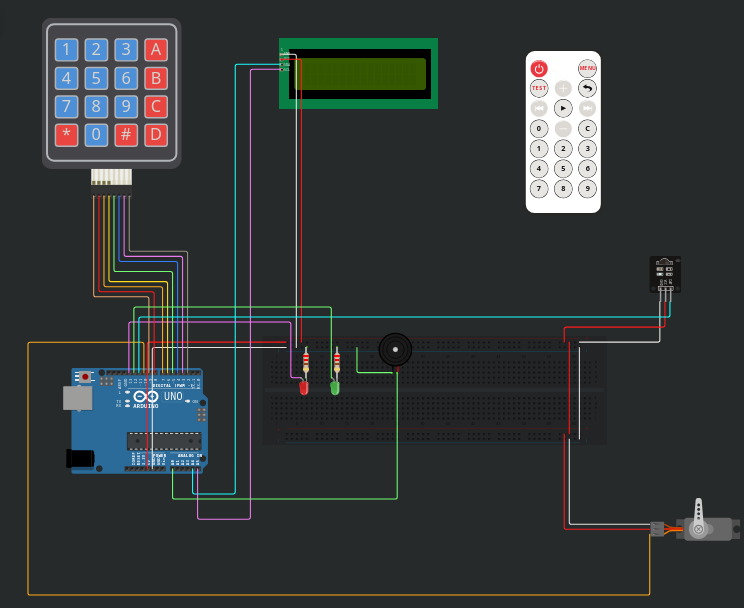
\includegraphics[width=0.48\textwidth]{simulacion.png}
    \caption{Simulación general del sistema de acceso seguro.}
    \label{fig:simulacion}
\end{figure}

\section{Montaje Físico}

Posteriormente se realizó el montaje físico del circuito utilizando protoboard y los componentes 
electrónicos seleccionados.

\begin{figure}[H]
    \centering
    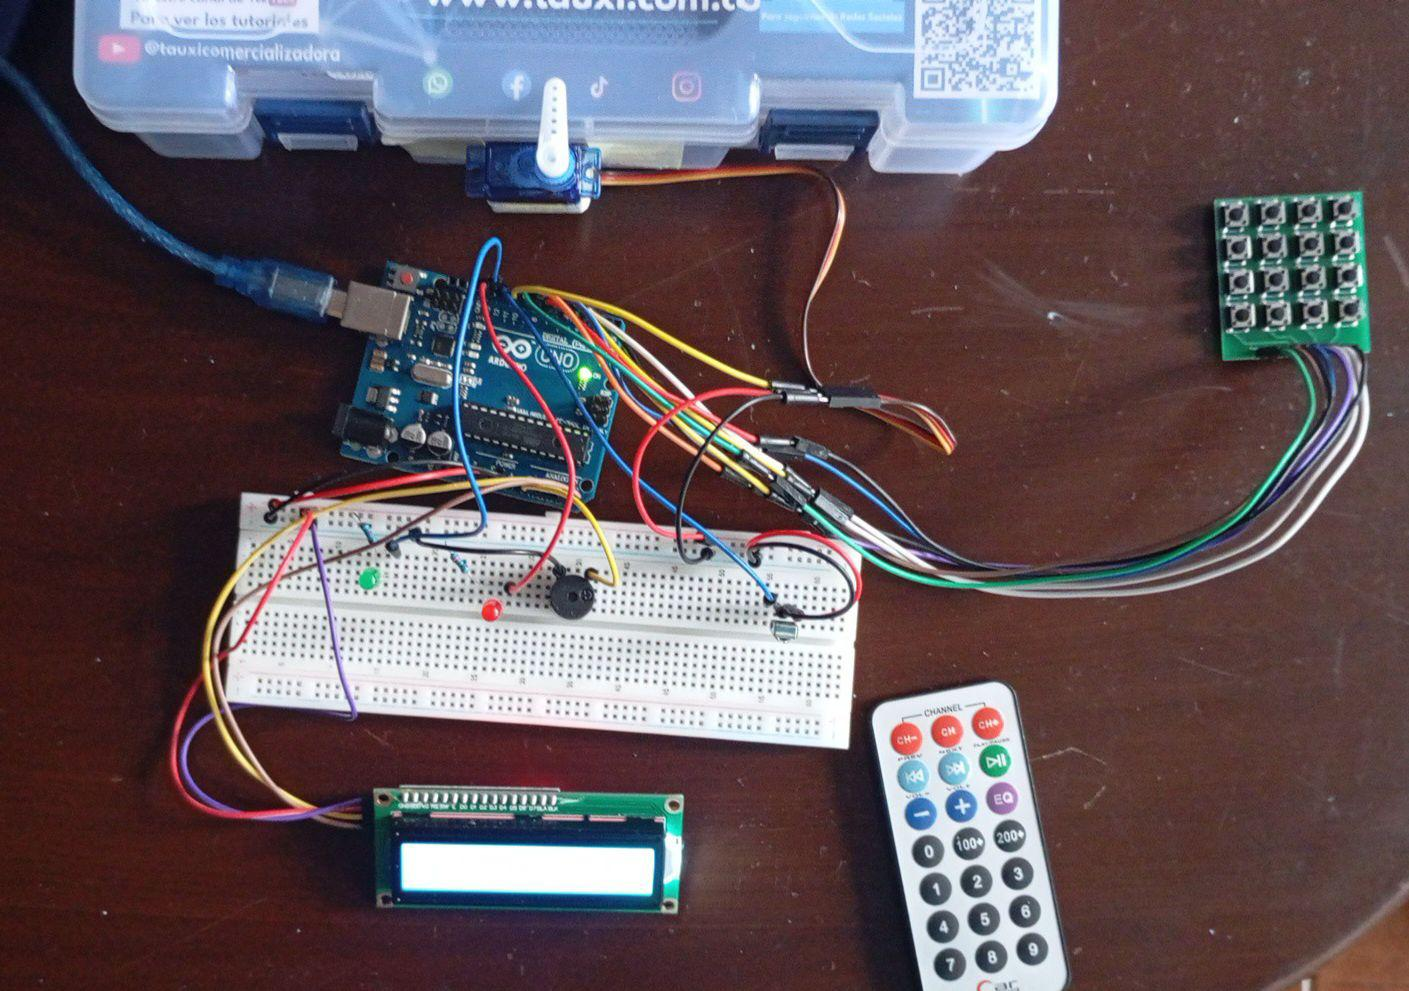
\includegraphics[width=0.48\textwidth]{montaje_fisico.jpeg}
    \caption{Montaje físico completo del proyecto.}
    \label{fig:montaje}
\end{figure}

\section{Interfaz del Sistema}

\subsection{Pantalla Inicial}

\begin{figure}[H]
    \centering
    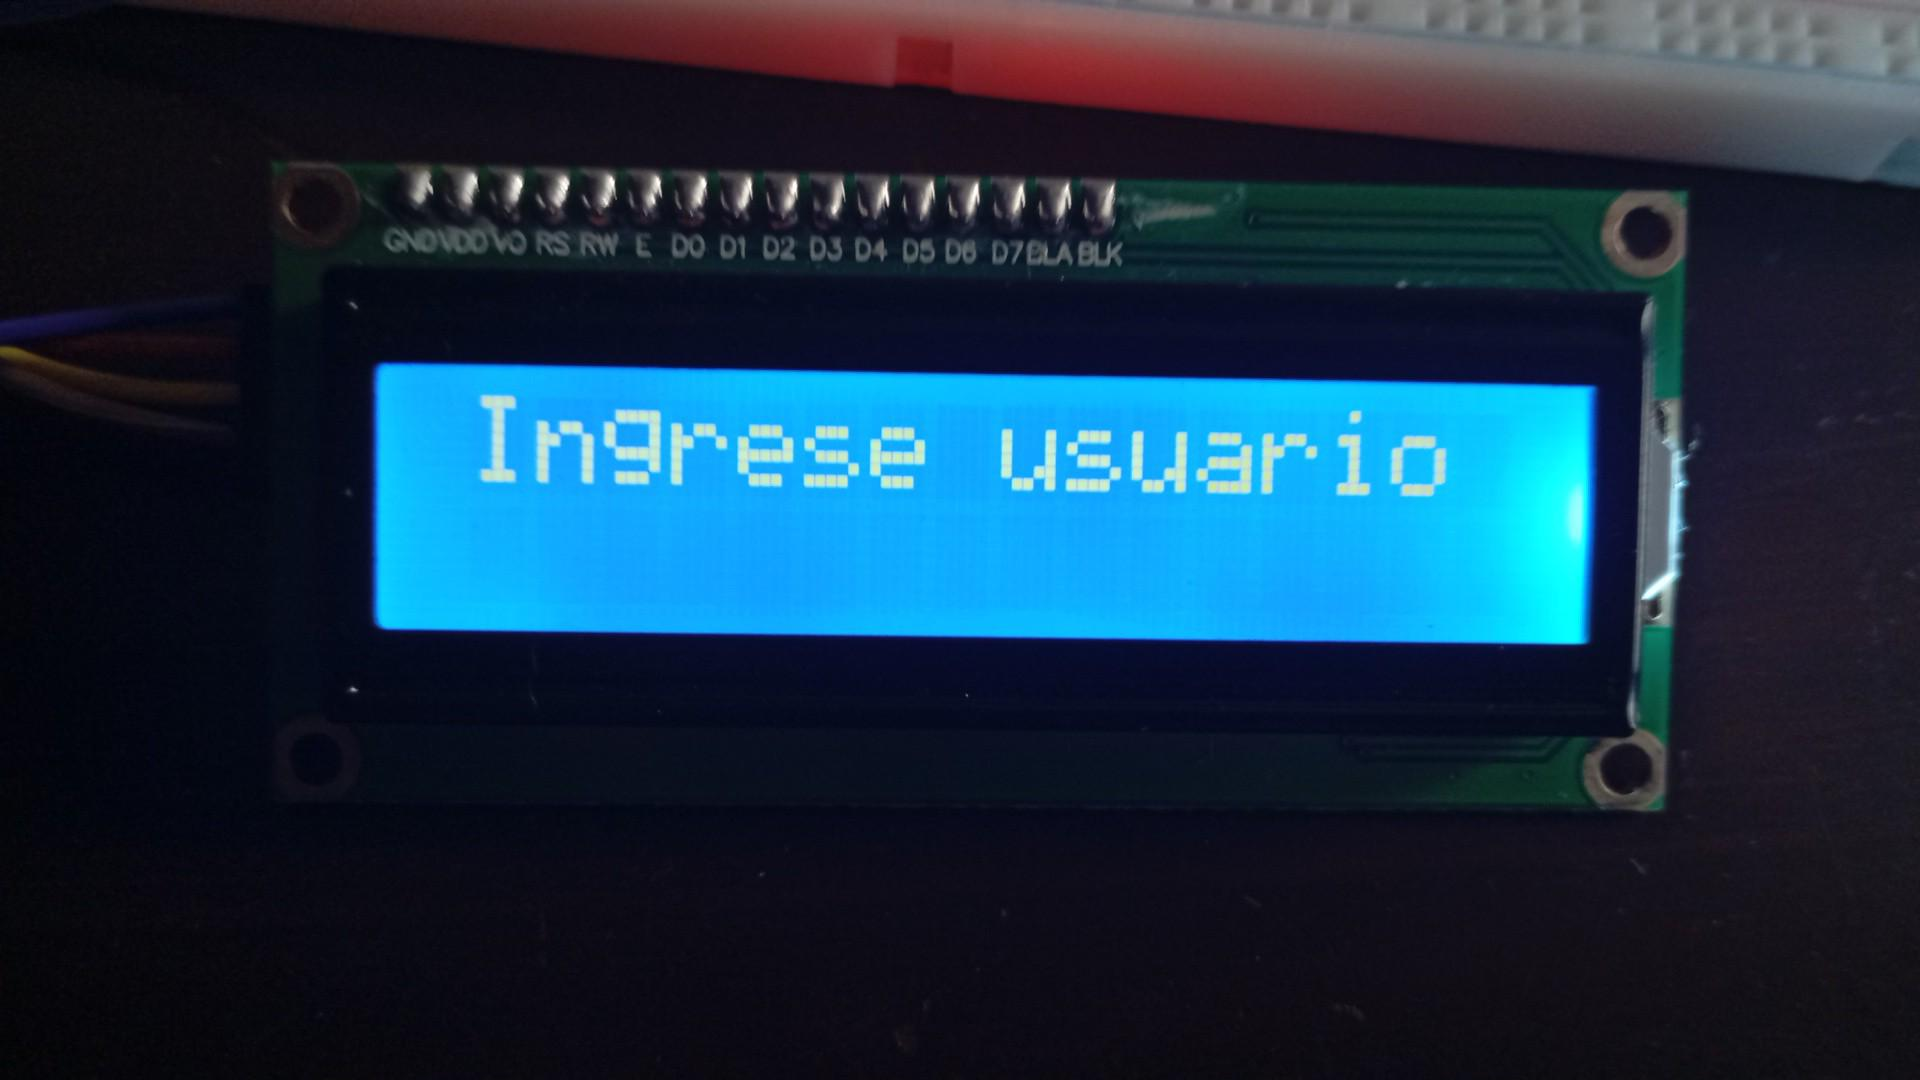
\includegraphics[width=0.35\textwidth]{pantalla_inicio.jpeg}
    \caption{Pantalla inicial del sistema.}
    \label{fig:inicio}
\end{figure}

\subsection{Acceso Permitido}

\begin{figure}[H]
    \centering
    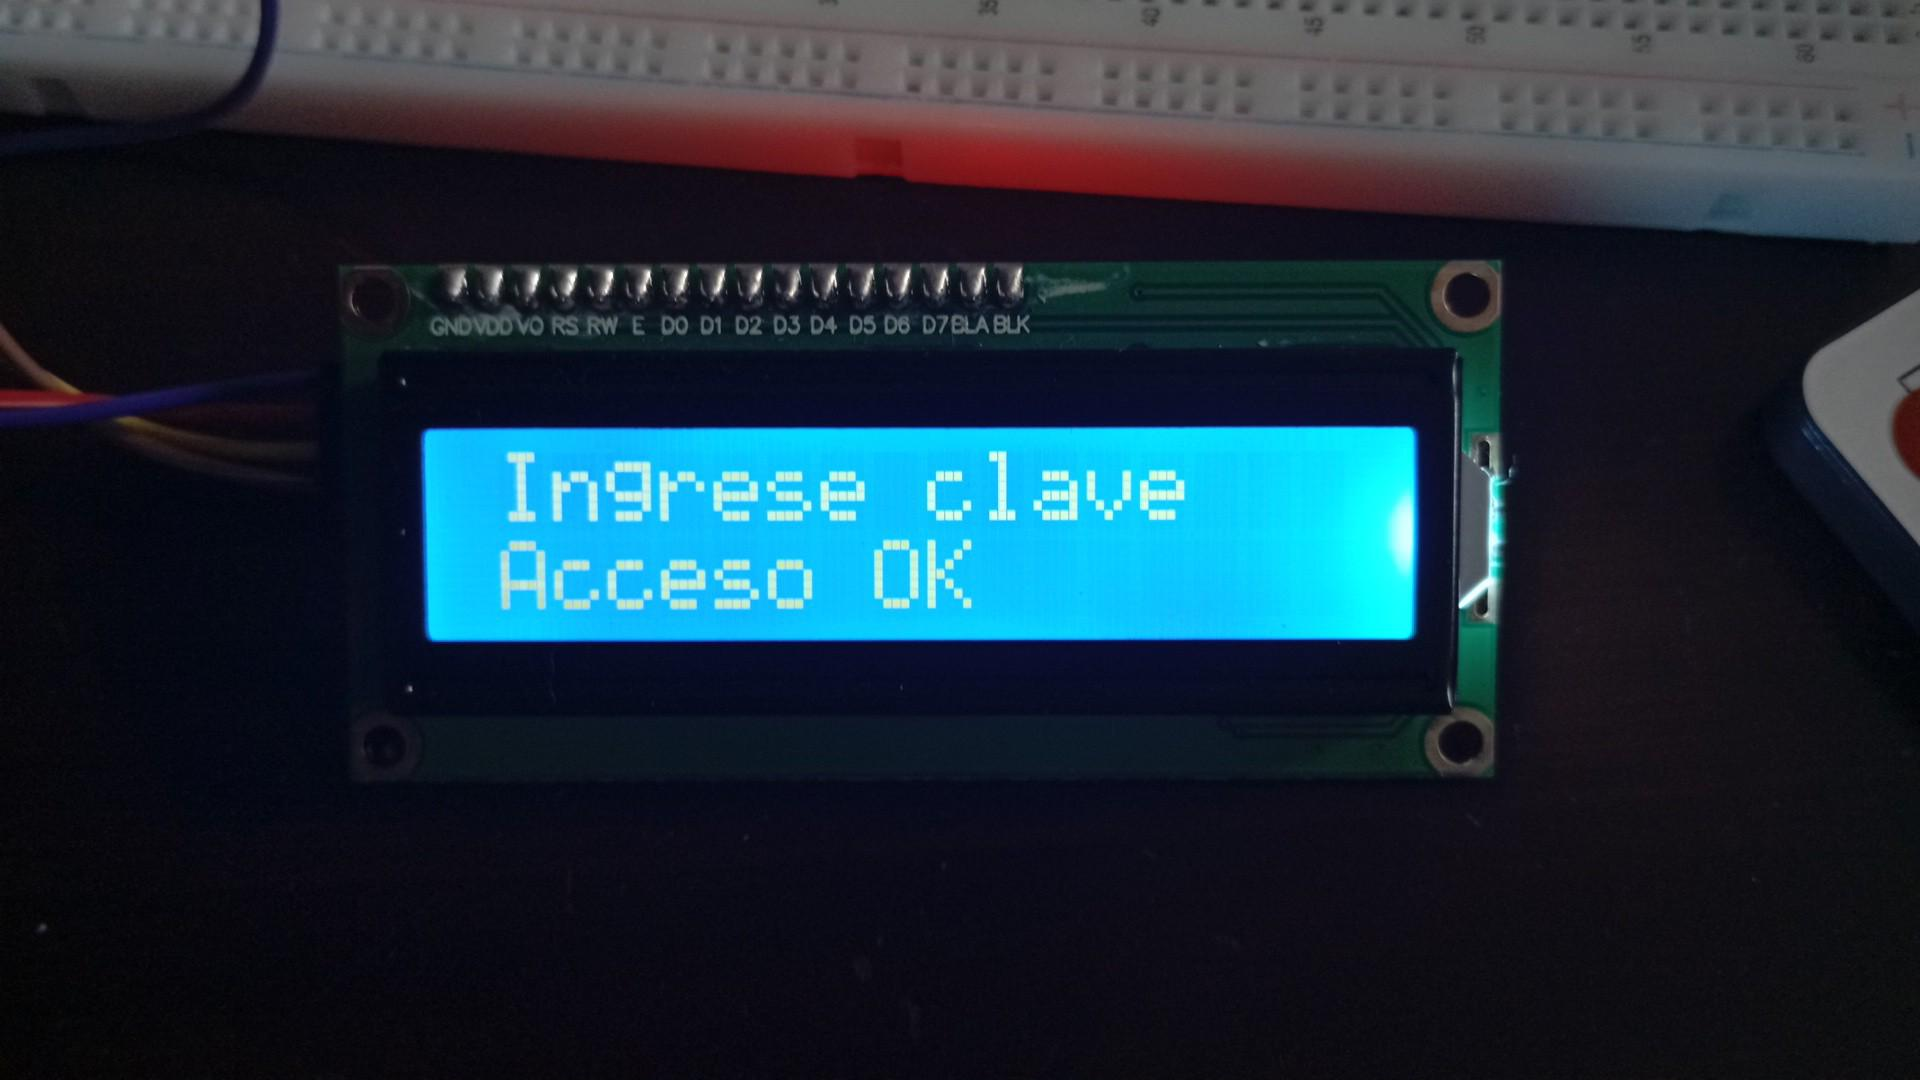
\includegraphics[width=0.35\textwidth]{acceso_permitido.jpeg}
    \caption{Mensaje de acceso permitido.}
    \label{fig:permitido}
\end{figure}

\subsection{Acceso Denegado}

\begin{figure}[H]
    \centering
    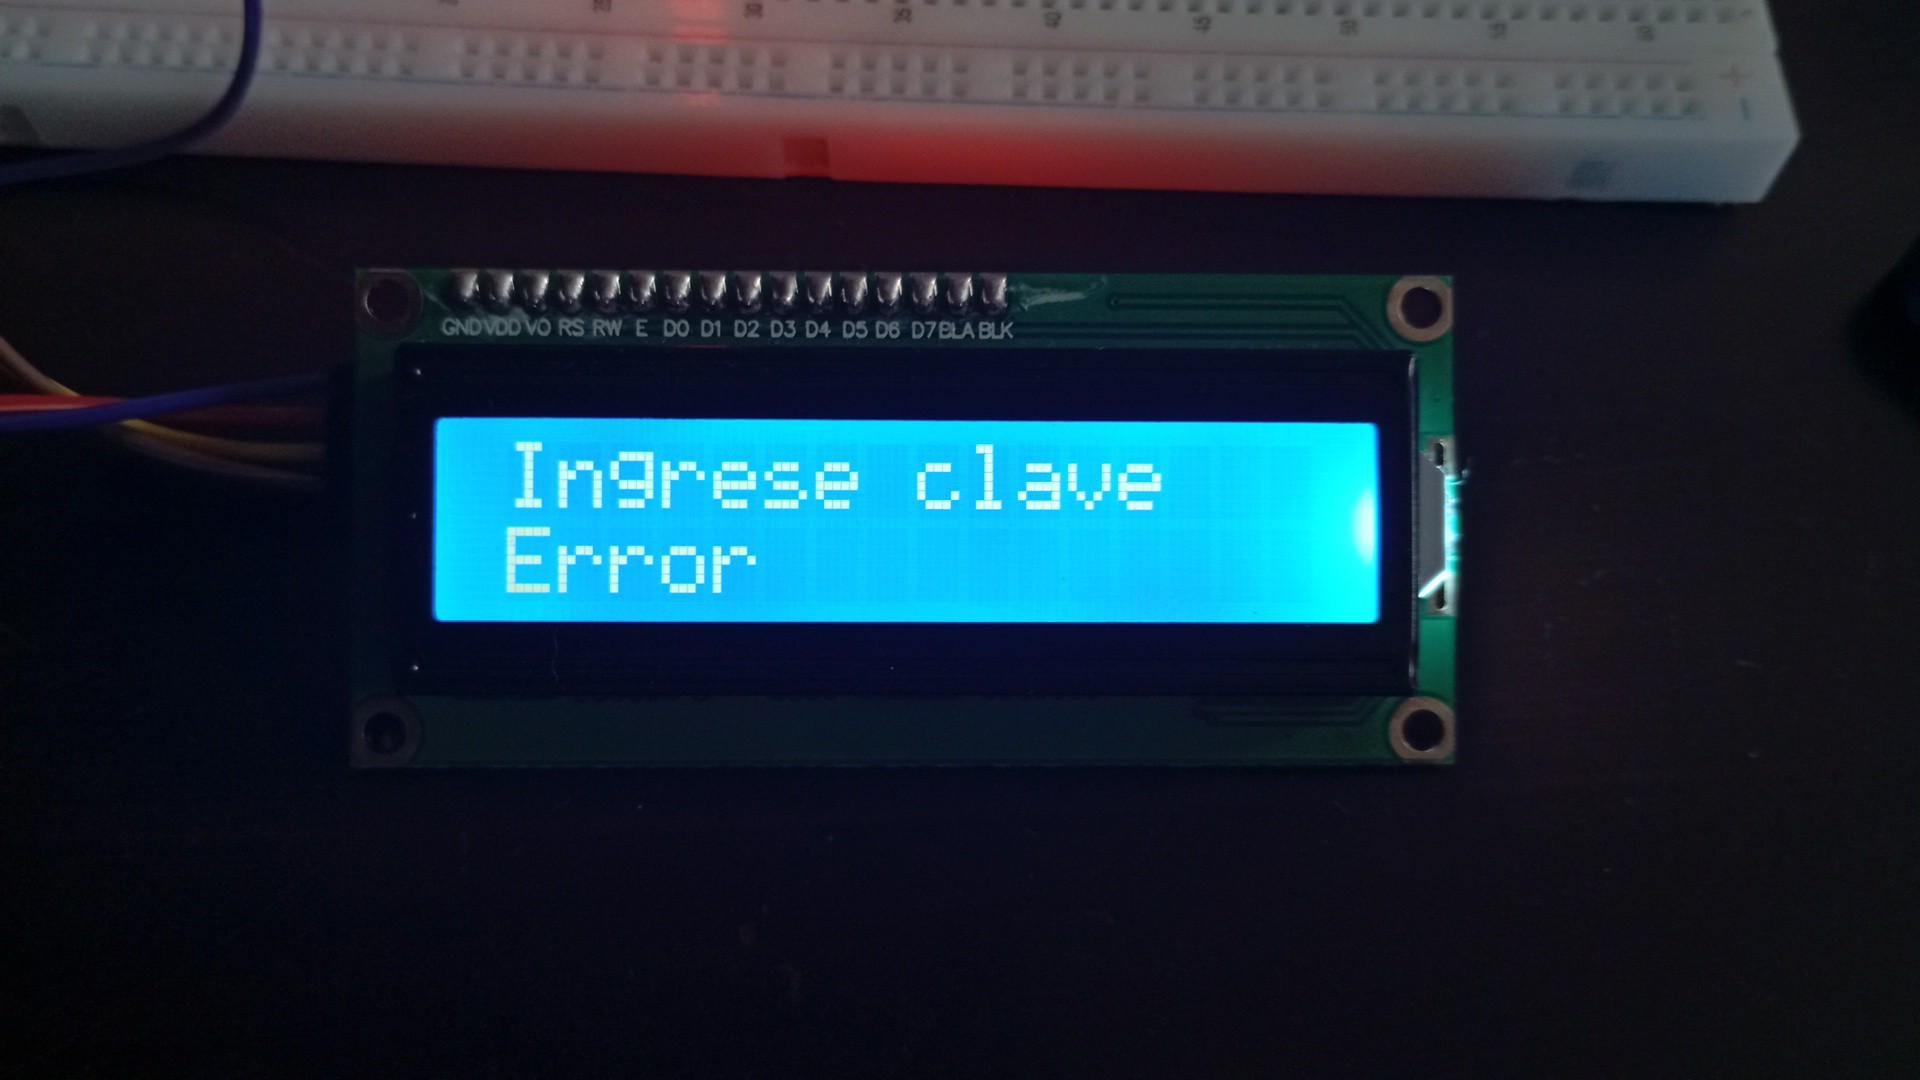
\includegraphics[width=0.35\textwidth]{acceso_denegado.jpeg}
    \caption{Mensaje de acceso denegado.}
    \label{fig:denegado}
\end{figure}

\subsection{Bloqueo Temporal}

\begin{figure}[H]
    \centering
    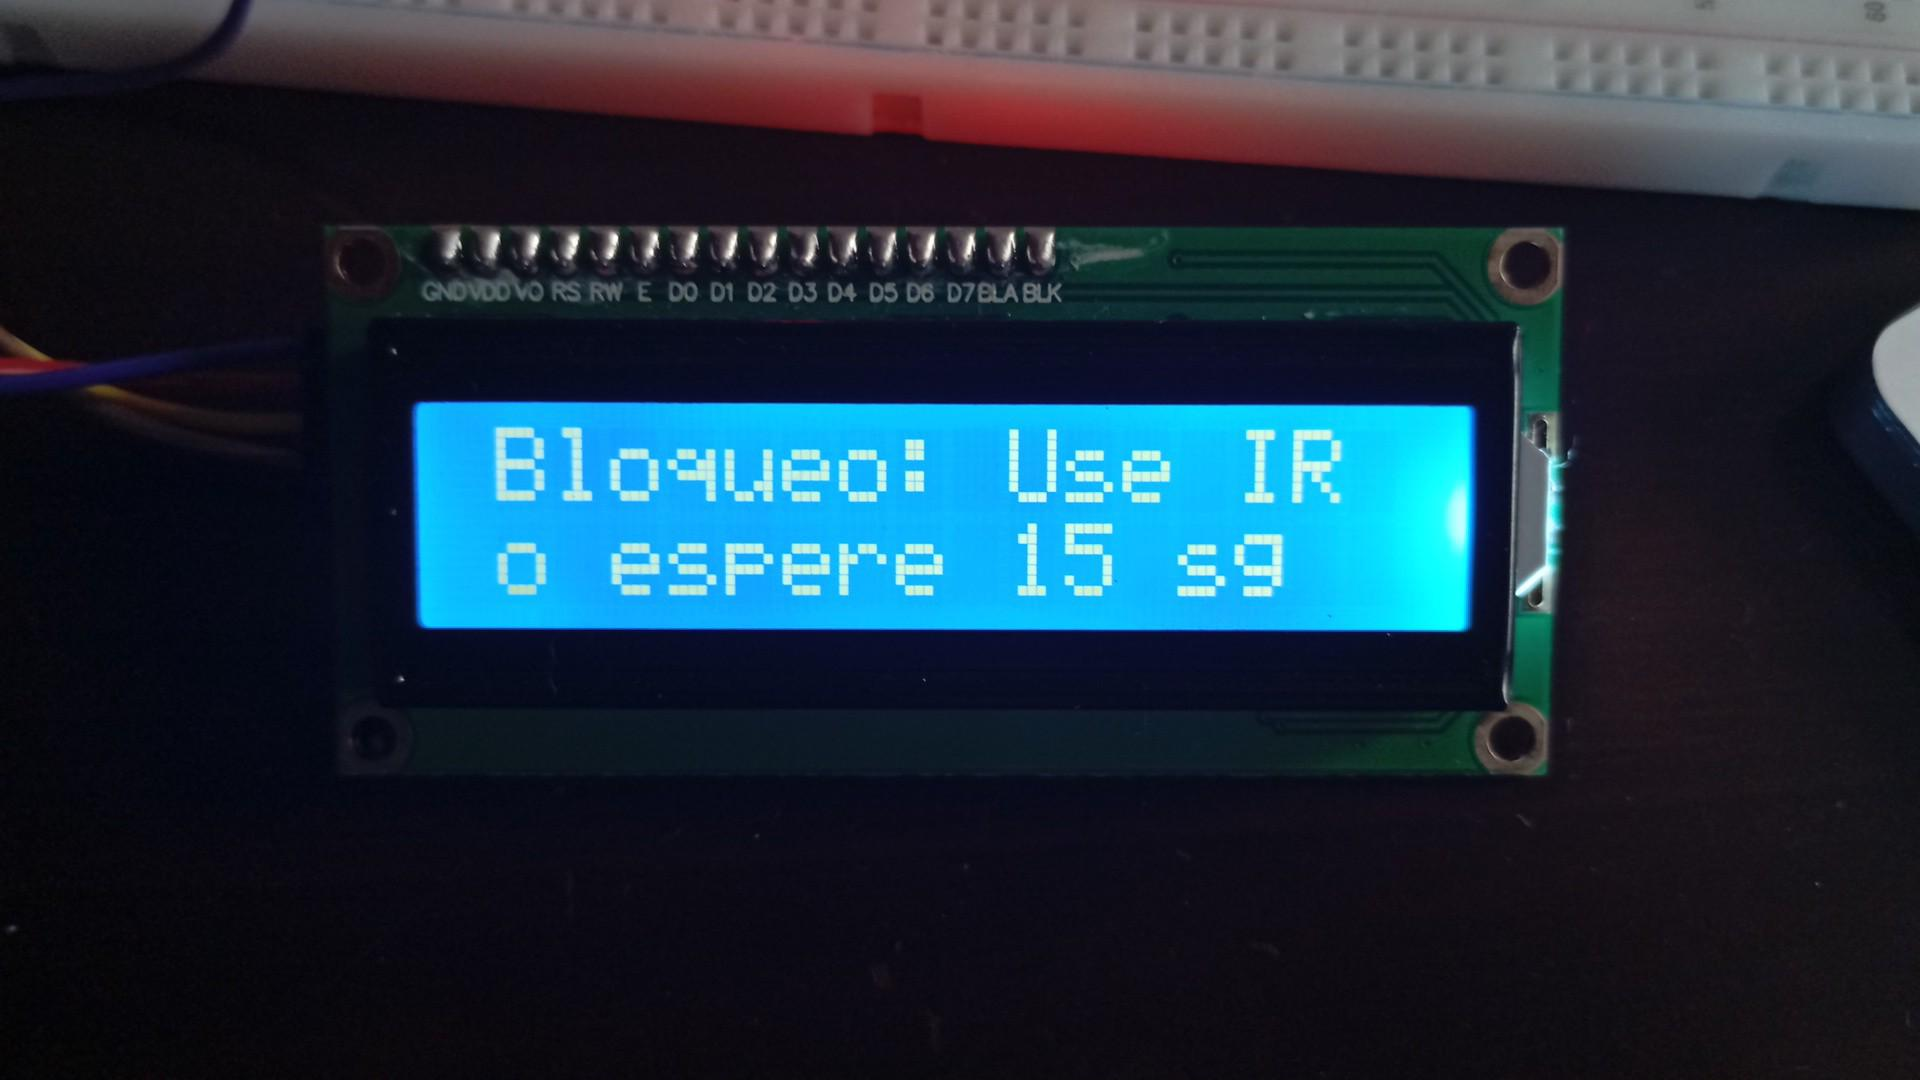
\includegraphics[width=0.35\textwidth]{bloqueo_temporal.jpeg}
    \caption{Mensaje de bloqueo temporal.}
    \label{fig:bloqueo}
\end{figure}

\section{Resultados}

El sistema desarrollado logró cumplir satisfactoriamente los objetivos planteados. Se consiguió 
implementar un mecanismo funcional de autenticación con apertura automática y alertas de seguridad.

Durante las pruebas realizadas se verificó el correcto funcionamiento de:

\begin{itemize}
    \item Ingreso y validación de clave.
    \item Apertura y cierre mediante servomotor.
    \item Alarmas sonoras y visuales.
    \item Bloqueo temporal por múltiples intentos fallidos.
    \item Visualización de mensajes en pantalla LCD.
    \item Funcionamiento simultáneo de módulos usando millis().
\end{itemize}

\section{Conclusiones}

El proyecto permitió integrar diferentes conceptos de programación y electrónica aplicada utilizando 
Arduino UNO.

Se evidenció la importancia de optimizar recursos en sistemas embebidos, especialmente en el manejo de 
memoria y temporizadores.

La implementación de lógica de estados y programación modular facilitó el desarrollo del sistema y 
mejoró la organización del código.

Finalmente, el proyecto demuestra cómo es posible desarrollar sistemas básicos de seguridad electrónica 
utilizando componentes de bajo costo y fácil acceso.

\section{Repositorio del Código Fuente}

El código fuente completo del proyecto se encuentra disponible en el siguiente repositorio de GitHub:

\vspace{0.3cm}

\noindent
\textbf{Repositorio GitHub:}

\url{https://github.com/KevinRCorrales/tex_informes/tree/main/automatas/momento3}

\vspace{0.3cm}

\noindent
En el repositorio se incluye:

\begin{itemize}
    \item Código fuente completo.
    \item Librerías utilizadas.
    \item Archivos de simulación.
    \item Documentación adicional.
\end{itemize}

\section{Video Demostrativo}

El funcionamiento completo del proyecto fue documentado mediante un video demostrativo subido a YouTube.

\vspace{0.3cm}

\noindent
\textbf{Enlace del video:}

\url{https://youtu.be/7yyA0VXawdo?si=rcZWxhE19kewvuIg}

\vspace{0.3cm}

\noindent
El video presenta:

\begin{itemize}
    \item Explicación general del sistema.
    \item Funcionamiento del ingreso de clave.
    \item Apertura mediante servomotor.
    \item Funcionamiento del buzzer y LEDs.
    \item Demostración del bloqueo temporal.
    \item Explicación del código y módulos utilizados.
\end{itemize}

\section*{Anexos}

\begin{itemize}
    \item Simulación del circuito.
    \item Código fuente en Arduino IDE.
    \item Evidencias fotográficas.
    \item Video demostrativo.
\end{itemize}

\begin{thebibliography}{00}

\bibitem{b3} Datasheet SG90 Servo Motor.

\bibitem{b4} Datasheet LCD 1602 I2C.

\bibitem{b5} Arduino Documentation, ``millis() Function,'' Disponible en: https://docs.arduino.cc/

\end{thebibliography}

\end{document}
